\documentclass[12pt]{article}
\usepackage[brazil]{babel}
\usepackage{graphicx}
\usepackage{mathtools}
\usepackage{float} 
\usepackage{xcolor}
\usepackage{amsmath, amssymb, bm}


\usepackage{array}
\usepackage{booktabs}



% margenes
\usepackage[a4paper,left=3cm,right=3cm,top=3cm]{geometry}

%opening
\title{}
\author{}

\begin{document}

\begin{center}
	{\tiny {\normalsize {\large \textbf{Convecção}\\ Lista de exercicios 2\\
	
	\textbf{Cristian Herledy Lopez Lara}}}}
\end{center}

\subsection*{Exercício 2,19 livro texto}


\textbf{Considerando a análise de transferência de calor do problema 2.18 e levando em conta que L é longo o suficiente para que o fluxo de calor $q_{b}$ não dependa de L, Determinar: A) Se b aumenta a uma taxa de duas vezes, por qual fator $q_{b}$ aumentará? B) Calcule a razão $q_{B,w}/q_{B,a}$} \\



\textbf{Informações de entrada} 

Do problema 2,18:

\begin{equation}
	\begin{aligned}
		q_{B} = (T_{B} - T_{\infty})(hpkA)^{\frac{1}{2}}\ tanh\left[L(\frac{hp}{kA})^{\frac{1}{2}}\right] 
	\end{aligned}
\end{equation}

\begin{equation}
	\begin{aligned}
		\frac{hb}{k_{f}}=0,664Pr^{\frac{1}{3}}\left(\frac{U_{\infty }b}{\nu} \right)^{\frac{1}{2}} 
	\end{aligned}
\end{equation}

\begin{figure}[H]
	\centering
	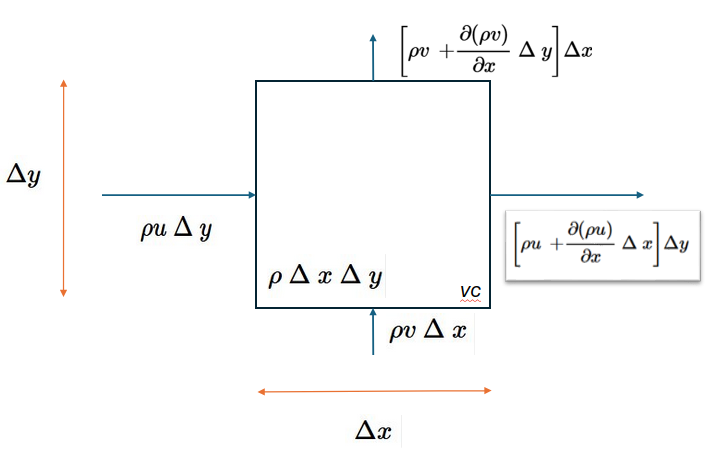
\includegraphics[width=.65\textwidth]{Figures/1_1}
	\caption{Transferência de calor em aleta com fluxo laminar paralelo a $b$.}
\end{figure}

Como $x\approx L$, supõe-se que seja longo o suficiente para não influenciar o comportamento de $q_{B}$, então $tanhL\rightarrow1$ na equaçao (1)

\begin{equation}
	\begin{aligned}
		q_{B} = (T_{B} - T_{\infty})(hpkA)^{\frac{1}{2}}\  
	\end{aligned}
\end{equation}

Considerando que $p=2b$, $A=bt$ e calculando h de (2):



\begin{equation}
	\begin{aligned}
		q_{B} = (T_{B} - T_{\infty})\left(\frac{0,664Pr^{\frac{1}{3}}k_{f}kbt2b}{b}\left(\frac{U_{\infty}b}{\nu}\right)^{\frac{1}{2}}\right)^{\frac{1}{2}}\  
	\end{aligned}
\end{equation}
\textbf{Item A}

A partir da equaçao (4), a relação entre $q_{b}$ e $b$ é encontrada 

\begin{equation}
	\begin{aligned}
		q_{B} = (T_{B} - T_{\infty})\left(1,328Pr^{\frac{1}{3}}k_{f}kt\left(\frac{U_{\infty}}{\nu}\right)^{\frac{1}{2}}\right)^{\frac{1}{2}} b^{\frac{3}{4}} 
	\end{aligned}
\end{equation}

Por tanto, $q_{B}$ é proporcional a $b$ na forma

\begin{equation}
	\begin{aligned}
		q_{B} \sim b^{\frac{\scriptstyle 3}{\scriptstyle 4}}
	\end{aligned}
\end{equation}
\begin{equation}
	\begin{aligned}
		q_{B} \sim 2^{\frac{\scriptstyle 3}{\scriptstyle 4}} = 1,68
	\end{aligned}
\end{equation}

Quando a altura da aleta é \textbf{dobrada}, a taxa de transferência de calor \textbf{aumenta em 68\%}
\\

\textbf{Item B}

Os radios podem ser calculados substituindo as propriedades de cada fluido na equação (5)

\begin{equation}
	\begin{aligned}
		\frac{q_{B,w}}{q_{B,a}} = \frac{(T_{B} - T_{\infty})\left(1,328Pr^{\frac{1}{3}}_{w}k_{w}kt\left(\frac{U_{\infty}}{\nu_{w}}\right)^{\frac{1}{2}}\right)^{\frac{1}{2}} b^{\frac{3}{4}} }{(T_{B} - T_{\infty})\left(1,328Pr^{\frac{1}{3}}_{a}k_{a}kt\left(\frac{U_{\infty}}{\nu_{a}}\right)^{\frac{1}{2}}\right)^{\frac{1}{2}} b^{\frac{3}{4}} }
	\end{aligned}
\end{equation}

Propriedades do escoamento como a velocidade, temperatura e volume, são constantes para cada caso. A razões totales podem ser calculadas a partir das razões das propriedades do fluido                    .

\begin{equation}
	\begin{aligned}
		\frac{q_{B,w}}{q_{B,a}} = \frac{\left(Pr^{\frac{1}{3}}_{w}k_{w} \nu^{-\frac{1}{2}}_{w}\right)^{\frac{1}{2}}  }{\left(Pr^{\frac{1}{3}}_{a}k_{a}\nu^{-\frac{1}{2}}_{a}\right)^{\frac{1}{2}}  }\ \ = \ \ \left( \frac{Pr_{w}}{Pr_{a}}\right)^{\frac{1}{6}} \left( \frac{\nu_{a}}{\nu_{w}}\right)^{\frac{1}{4}} \left( \frac{k_{a}}{k_{w}}\right)^{\frac{1}{2}}
	\end{aligned}
\end{equation}

\begin{equation}
	\begin{aligned}
		 \left( \frac{7}{0,72}\right)^{\frac{1}{6}} \left( {\frac{1}{0,07}}\right)^{\frac{1}{4}} \left( 23\right)^{\frac{1}{2}} = 13,5
	\end{aligned}
\end{equation}

Concluindo, a taxa de transferência de calor na água é aproximadamente \textbf{13 vezes maior} que no ar.

\subsection*{Exercício 2,23 livro texto}


\textbf{Com base na velocidade U e grossura do jet D do problema 2.22, calcule a ordem de magnitude de Dt e T para fluidos com $Pr >> 1$ e $Pr << 1$}. \\

\textbf{Informações de entrada}

\begin{equation}
	\frac{D_T(x)}{D(x)} \sim \text{Pr}^{-1/2}
\end{equation}

\begin{equation}
	\frac{T(x) - T_\infty}{T_0 - T_\infty} \sim \left( \frac{U_0 D_0 / \nu}{x / D_0} \right)^{1/3} \text{Pr}^{1/2} \ \ \text{(Pr } \gg 1 \text{)}
\end{equation}


\begin{equation}
	\frac{T(x) - T_\infty}{T_0 - T_\infty} \sim \left( \frac{U_0 D_0 / \nu}{x / D_0} \right)^{1/3} \ \ \text{(Pr } \ll 1 \text{)}
\end{equation}

 
\begin{figure}[H]
	\centering
	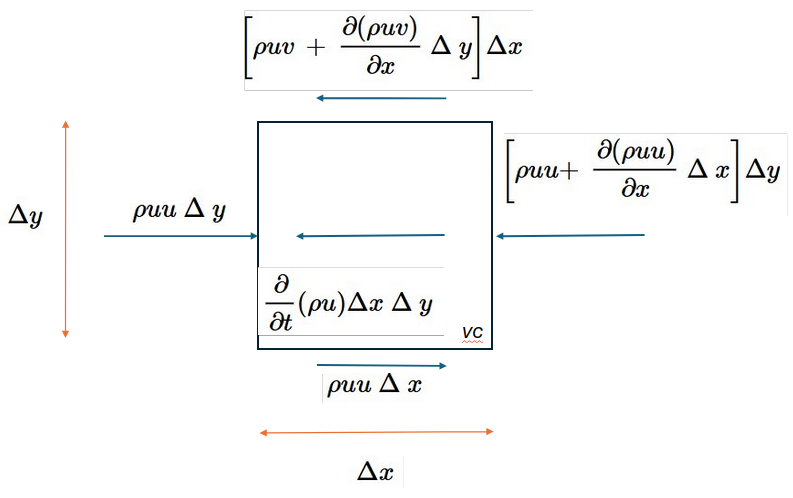
\includegraphics[width=.65\textwidth]{Figures/1_2}
	\caption{Esquema de camada limite hidrodinâmica e térmica em fluxo de jato}
\end{figure}

Do problema 2,22:

\begin{equation}
	\begin{aligned}
		\frac{D(x)}{D_{0}} \sim \left( \frac{x/D_{0}}{U_{0}D_{0}/\nu} \right) ^{\frac{2}{3}}
	\end{aligned}	
\end{equation}
\begin{equation}
	\begin{aligned}
		\frac{U(x)}{U_{0}} \sim \left( \frac{x/D_{0}}{U_{0}D_{0}/\nu} \right) ^{\frac{1}{3}}
	\end{aligned}	
\end{equation}
\textbf{Desenvolvimiento}

Primeiro, a equação de energia para a camada limite é estabelecida. Nesta equação, o termo associado aos efeitos da dufusividade em x é negligenciado.

\begin{equation}
	\begin{aligned}
		u\frac{\partial T}{\partial x} + v\frac{\partial T}{\partial y} = \alpha\left( \frac{\partial^{2} T}{\partial y^{2}}\right)
	\end{aligned}
\end{equation}

Fazendo a análise de escala obtem-se

\begin{equation}
	\begin{aligned}
		u\frac{\Delta T}{ x} + v\frac{\Delta T}{D_{T}} \sim \alpha\left( \frac{\Delta T}{D^{2}_{T}}\right)
	\end{aligned}
\end{equation}

Da equação de conservação de massa

\begin{equation}
	\begin{aligned}
		\frac{\partial u}{ \partial x} + \frac{\partial v}{\partial y} = 0 \ \rightarrow \frac{U}{x} \sim \frac{v}{D_{T}}
	\end{aligned}
\end{equation}
A equação (11) é reduzida a

\begin{equation}
	\begin{aligned}
		U\frac{\Delta T}{ x} \sim \alpha\left( \frac{\Delta T}{D^{2}_{T}}\right)
	\end{aligned}
\end{equation}

Com esta relação, pode-se calcular a razão entre as camadas limites hidrodinâmica e térmica

\begin{equation}
	\begin{aligned}
		\frac{D_{T}(x)}{D(x)} = \frac{x^{\frac{1}{2}}  \alpha^{\frac{1}{2}}  \nu^{\frac{1}{6}}   x^{\frac{1}{6}} / U^{\frac{2}{3}}_{0}  D^{\frac{1}{3}}_{0}  }         {U^{\frac{2}{3}}_{0}  D^{\frac{1}{3}}_{0}  / \nu^{\frac{2}{3}}   x^{\frac{2}{3}} } \ = \frac{\alpha^{\frac{1}{2}}}{\nu^{\frac{1}{2}}} \ = Pr^{\frac{1}{2}}
	\end{aligned}
\end{equation}

A equação (11) é satisfeita. Esta expressão mostra como o número de Prandtl é proporcional às dimensões das camadas limites. Agora, avaliamos como a temperatura muda ao longo do desenvolvimento da camada limite térmica. Invocando a integração da equação de energia

\begin{equation}
	\begin{aligned}
		\frac{\partial (uT)}{\partial x} + \frac{\partial (vT)}{\partial y} = \alpha\left( \frac{\partial^{2} T}{\partial y^{2}}\right)
	\end{aligned}
\end{equation}

Aplicando a fórmula integral de Leibniz

\begin{equation}
	\frac{d}{dx} \left[ \int_{-\infty}^{\infty} u T \, dy + T_\infty v_\infty - T_0 v_0 \right] = \alpha \left( \frac{\partial T}{\partial x} \bigg|_{y=\infty} - \frac{\partial T}{\partial x} \bigg|_{y=-\infty} \right)
\end{equation}

Como a temperatura fora da camada limite é a temperatura do reservatório, a variação de temperatura ao longo e dentro dessa zona é zero.

\begin{equation}
	\frac{d}{dx} \left[ \int_{-\infty}^{\infty} u T \, dy + T_\infty v_\infty - T_0 v_0 \right] = 0
\end{equation}

Para resolver o segundo e terceiro termos da integral, o balanço de massa é usado.

\begin{equation}
	\frac{\partial u}{\partial x} + \frac{\partial v}{\partial y} = 0
\end{equation}

\begin{equation}
	\int_{-\infty}^{\infty} \frac{\partial u}{\partial x} \, dy + \int_{-\infty}^{\infty} \frac{\partial v}{\partial y} \, dy = 0
\end{equation}

\begin{equation}
	\frac{d}{dx} \int_{-\infty}^{\infty} u \, dy + (v_\infty - v_{-\infty}) = 0
\end{equation}

\begin{equation}
	\frac{d}{dx} \int_{-\infty}^{\infty} u \, dy = -(v_\infty - v_{-\infty}) 
\end{equation}

Substituindo em (23)

\begin{equation}
	\frac{d}{dx} \int_{-\infty}^{\infty} u T \, dy - T_\infty \frac{d}{dx} \int_{-\infty}^{\infty} u \, dy = 0
\end{equation}

\begin{equation}
	\frac{d}{dx} \int_{-\infty}^{\infty} u (T - T_\infty) \, dy = 0
\end{equation}

É mostrado que o transporte de T na camada limite não depende de x. Como a expressão dentro da derivada (a integral) é constante
\begin{equation}
	\int_{-\infty}^{\infty} u (T - T_\infty) \, dy = \text{Constante} \sim  U_0 D_0 (\Delta T_{0})
\end{equation}

Onde $\Delta T_{0} = (T_{0} - T_\infty) $. Agora para a escala da integral

\begin{equation}
	\int_{-\infty}^{\infty} u (T - T_\infty) \, dy  \sim  U D_{geral} (\Delta T)
\end{equation}

Para determinar a escala $D_{geral}$, fazemos a análise de base com a escala de números de Prandtl indicada nas expressões (12) e (13)

\textbf{Caso 1: $Pr >> 1$}

\begin{equation}
	U \Delta T D \sim U_0 \Delta T_0 D_0
\end{equation}

\begin{equation}
	\Delta T \sim \frac{U_0 \Delta T_0 D_0}{U D}
\end{equation}

Das expressões (14) e (15), U e D são substituídos

\begin{equation}
	\Delta T \sim \frac{U_0 \Delta T_0 D_0}{\left( \frac{U_0^4 D_0^2}{v x} \right)^{1/3} \left( \frac{v x}{U_0 D_0^{1/2}} \right)^{2/3}}
\end{equation}

\begin{equation}
	\frac{\Delta T}{\Delta T_0} \sim \left( \frac{U_0 D_0^2}{v x} \right)^{1/3} 
\end{equation}

\textbf{Caso 2: $Pr << 1$}

\begin{equation}
	U \Delta T D_T \sim U_0 \Delta T_0 D_0
\end{equation}

\begin{equation}
	\Delta T \sim \frac{U_0 \Delta T_0 D_0}{U D_T}
\end{equation}

\begin{equation}
	\Delta T \sim \frac{U_0 \Delta T_0 D_0}{U D {Pr}^{-1/2}}
\end{equation}

\begin{equation}
	\frac{\Delta T}{\Delta T_0} \sim \left( \frac{U_0 D_0^2}{v x} \right)^{1/3}  {Pr}^{1/2}
\end{equation}
\\


\subsection*{Exercício solução de camada limite de Blasius}

Uma técnica comumente usada para resolver o problema do fluxo na camada limite é através do método de \textbf{similaridade} de Blasius. \\
Este método converte o problema de equações diferenciais parciais em um problema \textbf{não linear de equações ordinárias} de terceira ordem, usando uma variável de similaridade para os perfis \textbf{u e T}. A equação não linear será \textbf{resolvida numericamente}.\\


Matematicamente o perfil de velocidade é definido como

\begin{equation}
	\frac{u}{U_\infty} = \text{f}(\eta)
\end{equation}

Onde $\eta$ é proporcional a y por um fator dependente de x. $\eta$ será proporcional a

\begin{equation}
	\frac{u}{U_\infty} = f\prime  (\eta) \\
\end{equation}

\begin{equation}
	\eta = \frac{y}{x} \text{Re}_x^{1/2}
\end{equation}

O problema será regido pelas equações de conservação de massa (24) e momento (43) para a camada limite

\begin{equation}
	u \frac{\partial u}{\partial x} + v \frac{\partial u}{\partial y} = \nu \frac{\partial^2 u}{\partial y^2}
\end{equation}

Com o método da similaridade o problema se reduz a

\begin{equation}
	2 f^{\prime\prime\prime} + f f^{\prime\prime} = 0
\end{equation}

\begin{equation}
	f' = f = 0 \quad \text{at} \quad \eta = 0
\end{equation}

\begin{equation}
	f' \to 1 \quad \text{as} \quad \eta \to \infty
\end{equation}

A solução da equação fornece o perfil de velocidade na camada limite $f\prime$ e a tensão de cisalhamento. \\
Neste trabalho será dada uma solução numérica ao problema com o cálculo das derivadas com diferenças finitas da forma

\begin{equation}
	f' = \frac{f_{i+1} - f_i}{\Delta \eta}
\end{equation}

\begin{equation}
	f'' = \frac{f'_{i+1} - f'_i}{\Delta \eta}
\end{equation}

\begin{equation}
	f''' = \frac{f''_{i+1} - f''_i}{\Delta \eta}
\end{equation}

Os cálculos na etapa de iteração i+1 serão avaliados com base na etapa anterior de acordo com as expressões

\begin{equation}
	f_{i+1} = f_i + (\Delta \eta) f'_i
\end{equation}

\begin{equation}
	f'_{i+1} = f'_i + (\Delta \eta) f''_i
\end{equation}

\begin{equation}
	f''_{i+1} = f''_i + (\Delta \eta) f'''_i
\end{equation}
E da equação (44)

\begin{equation}
	f_i''' = -\frac{f_i f_i''}{2}
\end{equation}
\\

A solução obtida neste trabalho foi alcançada fazendo espaçamentos de domínio de $\eta = 0,01$. Diferentes valores estimados para $f\prime\prime$ ($0,2 < f\prime\prime < 0.8$) foram testados. \\
 
 O cálculo foi feito ate $\eta \sim 6$ para garantir o valor de $U\infty$ de acordo com a condição de contorno (46).
 
 \begin{figure}[H]
 	\centering
 	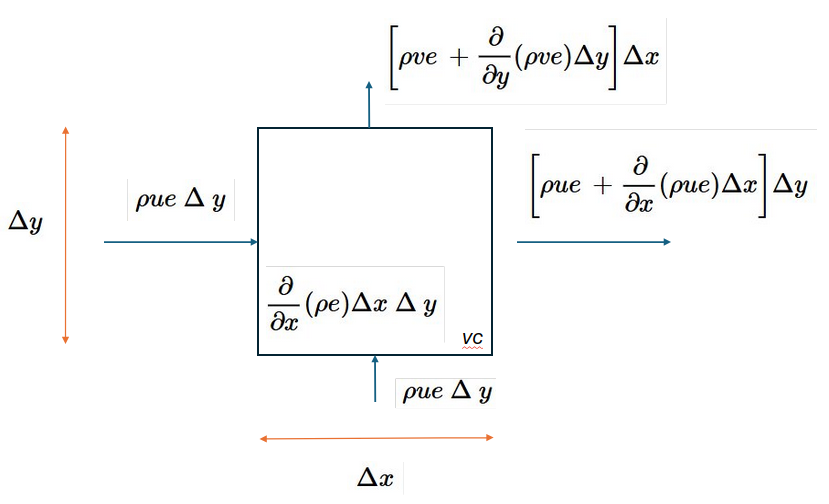
\includegraphics[width=.65\textwidth]{Figures/1_4}
 	\caption{Exemplo de tabela para cálculo numérico do perfil de velocidade}
 \end{figure}
 
 
 \textbf{Análise e conclusão}
 
 O resultado com convergência mais estável foi o valor de referência de $f\prime\prime =0,332$. Com este valor, A solução numérica mostrou que $u=0,99U_{\infty}$ foi atingido com $\eta = 4,98$.\\
 
 Na imagem a seguir, pode-se ver graficamente como a razão de velocidade $f\prime$ em relação à variável de similaridade $\eta$ converge para 1 quando $u$ tende a $U\infty$
 


\begin{figure}[H]
	\centering
	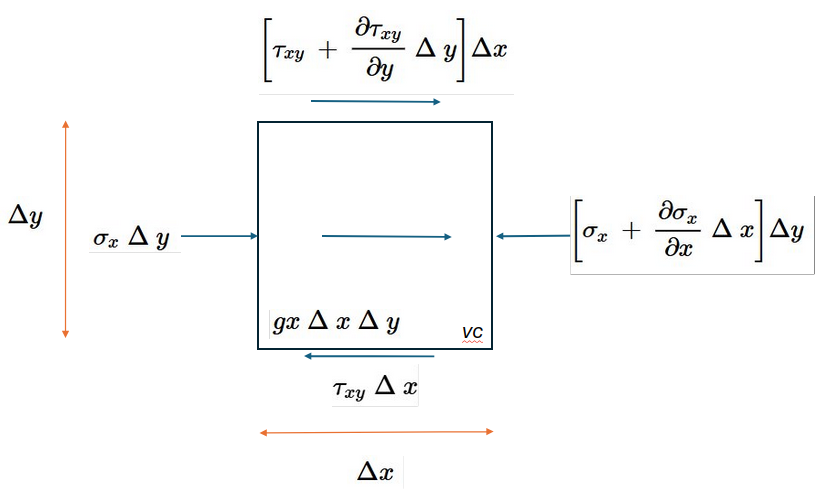
\includegraphics[width=.65\textwidth]{Figures/1_3}
	\caption{Perfil de velocidade na solução numérica da equação de Blasius}
\end{figure}

 Esta solução mostra um resultado correto em relação ao resultado de referência esperado em relação aos encontrados no problema 2.2 e na figura 2.6 do texto livro.





\end{document}





